% fixture: tikz/matrix-nodes
% tier: T3
% engine: document
% specials: compare
% covers: the matrix library: matrix of nodes with nodes in empty cells and a cell's |options|, matrix of math nodes, the cells' names in lines between them
\documentclass{article}
\usepackage{tikz}
\usetikzlibrary{matrix}
\begin{document}
Nodes 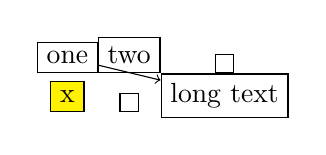
\begin{tikzpicture}
\matrix (m) [matrix of nodes, nodes={draw}, nodes in empty cells] { one & two & \\ |[fill=yellow]| x & & long text \\ };
\draw[->] (m-1-1) -- (m-2-3);
\end{tikzpicture} and \begin{tikzpicture}
\matrix (m) [matrix of math nodes, row sep=2em, column sep=3em] { A & B \\ C & D \\ };
\draw[->] (m-1-1) -- (m-1-2);
\draw[->] (m-1-1) -- node[left] {$f$} (m-2-1);
\end{tikzpicture} end.
\end{document}
